% Progress Report (D2, Hafta 7). 4-5 sayfa.
% Derleme (bu klasörden): latexmk -pdf progress.tex
% Şekil ve tablolar ../../results/ altından okunuyor; src/eda.py ile yeniden üretilir.

\documentclass[10pt,a4paper,twocolumn]{article}

\usepackage[utf8]{inputenc}
\usepackage[T1]{fontenc}
\usepackage[hmargin=1.6cm,top=1.4cm,bottom=1.6cm]{geometry}
\linespread{0.96}
\usepackage{times}
\usepackage{titlesec}
\usepackage{microtype}
\usepackage{url}
\urlstyle{same}
\usepackage{graphicx}
\graphicspath{{../../results/figures/}}
\usepackage{xcolor}
\usepackage{booktabs}
\usepackage{tikz}
\usetikzlibrary{arrows.meta,positioning}
\definecolor{atanavy}{HTML}{2A2660}
\usepackage[superscript]{cite}
\makeatletter
\renewcommand{\@citess}[1]{\textsuperscript{[#1]}}
\makeatother
\usepackage[hidelinks]{hyperref}
\usepackage[font=small,labelfont=bf,skip=4pt]{caption}

\titleformat{\section}{\normalsize\bfseries\color{atanavy}}{\thesection.}{0.5em}{}
\titlespacing*{\section}{0pt}{1.0ex plus 0.3ex}{0.5ex}
\titleformat{\paragraph}[runin]{\normalsize\bfseries}{}{0pt}{}[.]
\titlespacing*{\paragraph}{0pt}{0.6ex plus 0.2ex}{0.5em}
\setlength{\parskip}{0.3ex}

% Henüz yazılmamış yerler için gri not. Teslimden önce hepsi silinecek.
\newcommand{\todo}[1]{\textcolor{gray}{\textit{[TODO: #1]}}}

\title{\vspace{-1.6cm}
\includegraphics[height=1.3cm]{atauni-logo.png}\\[0.6em]\Large\textbf{Emotion-Driven VTuber Avatars: Progress Report}}
\author{Ömer Sunguralp Bektaş \\
\small Artificial Intelligence and Data Engineering, Atatürk University, Erzurum, Türkiye \\
\small \href{mailto:omersunguralp.bektas24@ogr.atauni.edu.tr}{omersunguralp.bektas24@ogr.atauni.edu.tr} \enspace$\cdot$\enspace ORCID: \href{https://orcid.org/0009-0000-8254-4949}{0009-0000-8254-4949}}
\date{}

\begin{document}
\maketitle

% 0. Kısa giriş + özet (Hafta 7, en son yazılır)
\section{Introduction}
\todo{Short summary of the project and of what this report covers. Written last, in week 7.}

% 1. Dataset analysis (Hafta 4 metin, Hafta 5 görseller)
% 1. Dataset analysis
% Kaynak: notlar.md (Kararlar, Veri seti gözlemleri). Sayılar results/ altındaki dosyalardan.
% Bütçe: ~1 sayfa (Hafta 5'te eklenecek görsellerle birlikte).

\section{Dataset Analysis}\label{sec:dataset}

\paragraph{Source and licence}
I use the RAVDESS dataset~\cite{ravdess}, downloaded from its official Zenodo record~\cite{ravdesszenodo}. It contains recordings of 24 professional actors (12 female, 12 male) who say two lexically matched sentences, ``Kids are talking by the door'' and ``Dogs are sitting by the door'', with different emotions. The recordings were made under controlled studio conditions, and their emotional content was validated by 247 raters in the original study~\cite{ravdess}. The dataset is released under the CC BY-NC-SA 4.0 licence. I use it only for this non-commercial course project and I do not redistribute it, so the video files are not part of the code repository. After downloading, I checked all 24 archives against the MD5 checksums published on Zenodo.

\paragraph{Selected subset}
Every RAVDESS recording exists in three versions: audio-visual (modality~01), video-only (02) and audio-only (03). Because this project uses only the visual modality, I kept only the video-only files. The audio-visual files contain exactly the same frames, so using them as well would count every clip twice. I also left out the song part of the dataset, because it covers only six of the eight emotions (surprise and disgust are missing) and has no recordings for one of the actors. The resulting subset has 1,440 clips, 60 per actor (Table~\ref{tab:dataset}). Each file name encodes the modality, emotion, intensity, sentence, repetition and actor, so I built the index of the dataset directly from the file names and checked all expected counts automatically.

\begin{table}[t]
\centering
\caption{Summary of the dataset used in this project.}
\label{tab:dataset}
\small
\begin{tabular}{@{}ll@{}}
\toprule
Property & Value \\
\midrule
Source & RAVDESS, Zenodo record 1188976 \\
Licence & CC BY-NC-SA 4.0 \\
Subset & Video-only (modality 02), speech \\
Actors & 24 (12 male, 12 female) \\
Clips & 1,440 (60 per actor) \\
Resolution & 1280$\times$720, H.264 \\
Frame rate & 29.97 fps \\
Clip length & 2.94--5.27 s (median 3.67 s) \\
Frames per clip & 88--158 (median 110) \\
Classes & 7 (calm merged into neutral) \\
Clips per class & neutral 288, others 192 each \\
Training set & 16 actors (960 clips) \\
Validation set & actors 3, 12, 21, 24 (240 clips) \\
Test set & actors 4, 6, 7, 23 (240 clips) \\
\bottomrule
\end{tabular}
\end{table}


All clips are H.264 videos with a resolution of $1280\times720$. Their measured frame rate is 29.97~fps (in the proposal I gave the nominal value of 30~fps). The clips are short, between 2.94 and 5.27~s (88--158 frames, median 110), so even the shortest clip has enough frames for the frame counts $T \in \{8, 16, 32\}$ that I plan to test.

\paragraph{Classes}
RAVDESS uses eight emotion labels. Every emotion except neutral is recorded at two intensities (normal and strong), with both sentences and two repetitions, which gives 8 clips per actor. Neutral is recorded only at normal intensity, so it has 4 clips per actor. As planned in the proposal, I merged calm into neutral, because both are low-arousal expressions that look very similar on the face and both correspond to a resting expression of the avatar. Figure~\ref{fig:classes} shows the class distribution before and after merging. The merged neutral class has 288 clips (96 neutral and 192 calm), while each of the other six classes has 192 clips. Neutral is therefore 1.5 times larger than the other classes and makes up 20\% of the data. Because of this imbalance, I use the macro F1-score, which gives every class the same weight, as the main metric. Within every class, half of the clips come from male and half from female actors, and except for neutral, half are at normal and half at strong intensity, so gender and intensity are balanced by design.

\begin{figure}[t]
\centering
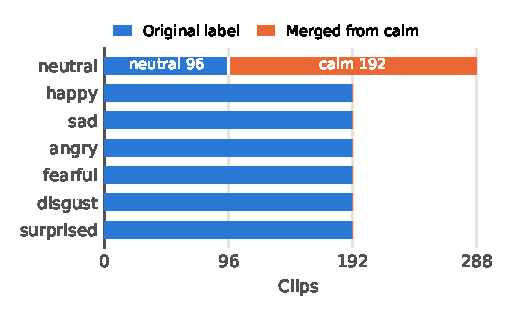
\includegraphics[width=\columnwidth]{class_distribution.pdf}
\caption{Number of clips per class. The neutral class is the union of the original neutral (96) and calm (192) clips.}
\label{fig:classes}
\end{figure}

% Hafta 5: her duygudan örnek yüz kırpması + bir klibin kare şeridi (tek şekil olarak birleştirilebilir)
% Hafta 5: klip süresi / kare sayısı histogramı
\todo{Week 5: sample face for each emotion, frame strip of one clip, clip length histogram.}

\paragraph{Actor-wise split}
To make sure that the models are always evaluated on faces they have not seen during training, I split the data by actor, so all clips of an actor are used for only one purpose. I first divided the 24 actors into six folds of four actors, two male and two female, using a fixed random seed (4206). In cross-validation round $k$, fold $k$ is the test set, fold $k+1$ (modulo~6) the validation set and the remaining four folds (16 actors) the training set, so every actor is in the test set exactly once. Because every actor has the same number of clips per emotion, every fold is also class-balanced (48 neutral clips and 32 clips of each other class). The fixed split used during development is round~0 of this cross-validation: actors 4, 6, 7 and 23 for testing, actors 3, 12, 21 and 24 for validation and the remaining 16 actors for training (960 / 240 / 240 clips). Using one round of the cross-validation as the fixed split makes the development results directly comparable with the final cross-validation results. The test actors are locked until model development is finished: the data loading code returns the test set only when this is requested explicitly, and all results in this report are on the validation actors.


% 2. Preprocessing (Hafta 5)
\section{Preprocessing}
\todo{Frame sampling, face detection, cropping, resizing, normalisation, augmentation; what and why for each step. Pipeline diagram.}

% 3. Baseline results (Hafta 6)
\section{Baseline Results}
\todo{Simple CNN: frame- and clip-level macro-F1 and accuracy on the validation actors, confusion matrix, loss curves, overfitting discussion.}

% 4. Initial DL model (Hafta 6)
\section{Initial Deep Learning Model}
\todo{Frame-based ResNet-18: architecture, replaced output layer, pretrained weights, training settings.}

% 5. Initial results (Hafta 7)
\section{Initial Results}
\todo{Comparison table: baseline vs.\ ResNet-18, short interpretation.}

% 6. Problems encountered (Hafta 7, notlar.md'den)
\section{Problems Encountered}
\todo{Group the entries of the problem log under 3--5 headings, with how each was or will be solved.}

% 7. Revised methodology + plan (Hafta 7)
\section{Revised Methodology and Remaining Plan}
\todo{What changed since the proposal and why; plan for the remaining weeks.}

{\small
\begin{thebibliography}{9}
\setlength{\itemsep}{0pt}

\bibitem{ravdess}
S.~R. Livingstone and F.~A. Russo, ``The Ryerson Audio-Visual Database of Emotional Speech and Song (RAVDESS): A dynamic, multimodal set of facial and vocal expressions in North American English,'' \emph{PLoS ONE}, vol.~13, no.~5, e0196391, 2018.

\bibitem{ravdesszenodo}
S.~R. Livingstone and F.~A. Russo, ``The Ryerson Audio-Visual Database of Emotional Speech and Song (RAVDESS),'' Zenodo, 2018. \url{https://doi.org/10.5281/zenodo.1188976}

\end{thebibliography}
}

\end{document}
